\documentclass[../TDM1-M2.tex]{subfiles}%

\begin{document}
\section[s]"1"{Charge soulevée par une grue}

\enonce{%
	Une grue de chantier de hauteur $h$ doit déplacer d'un point à un autre du
	chantier une charge M de masse $m$ supposée ponctuelle. On appelle A le point
	d'attache du câble sur le chariot de la grue.
	\smallbreak
	\noindent
	\begin{minipage}{0.45\linewidth}
		\begin{center}
			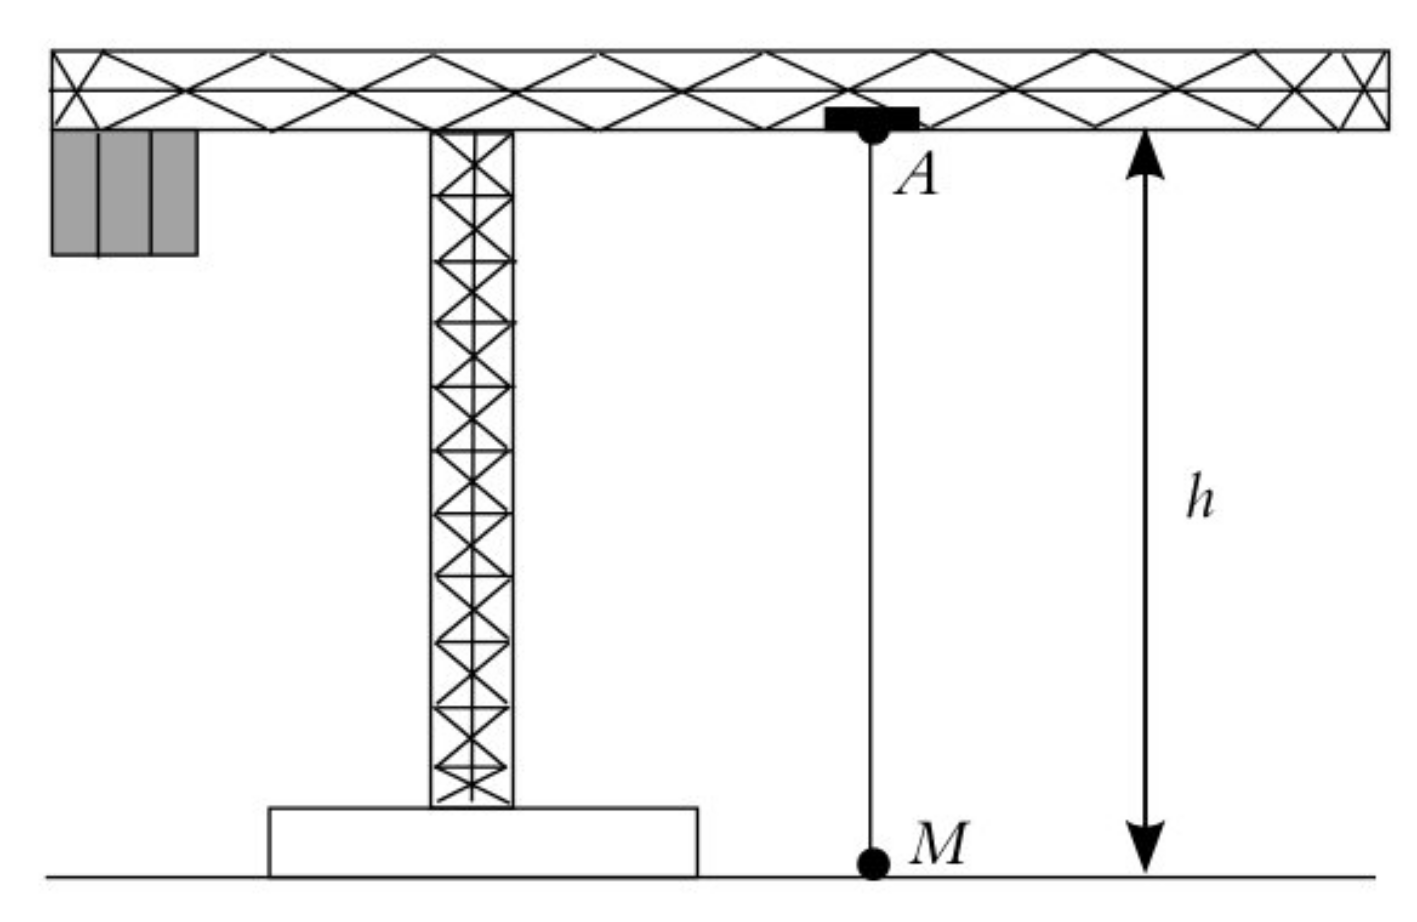
\includegraphics[height=3cm]{grue_fig1-plain}
			\captionof{figure}{Mouvement vertical}
			\label{fig:grue1_plain}
		\end{center}
	\end{minipage}
	\hfill
	\begin{minipage}{0.45\linewidth}
		\begin{center}
			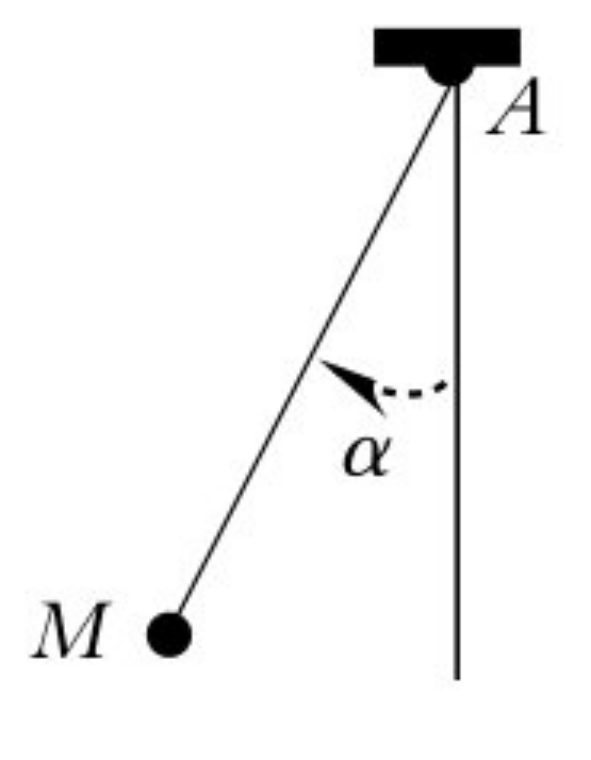
\includegraphics[height=3cm]{grue_fig2-plain}
			\captionof{figure}{Mouvement horizontal}
			\label{fig:grue2_plain}
		\end{center}
	\end{minipage}
}

\QR{%
	Le point A est à la verticale de M posée sur le sol. Déterminer la
	tension du câble lorsque M décolle (figure~\ref{fig:grue1_plain}).
}{%
	\begin{itemize}
		\item[b]{Système}~: \{masse $m$\} repérée par son centre d'inertie $M$.
		\item[b]{Référentiel}~: relié au sol, galiléen.
		\item[b]{Coordonnées}~: cartésiennes, $(\Or,\ux,\uy,\uz)$ avec $\uz$
		      vertical ascendant, O au pieds de la grue.
		\item[b]{BDF}~: avant qu'elle ne décolle, il y a la réaction du sol~; on
		      s'intéresse au décollage, donc au moment où elle s'annule. On
		      aura donc
		      \[
			      \begin{array}{ll}
				      \textbf{Poids}   & \Pf = m\gf = -mg\uz \\
				      \textbf{Tension} & \Tf = T\uz
			      \end{array}
		      \]

		\item[b]{PFD}~: au moment où la masse décolle, son accélération est
		      positive et selon $\uz$, soit $\af = \zpp\uz$~; en supposant un
		      décollage en douceur, $\zpp \approx 0$, soit
		      \[
			      m\af = \Pf + \Tf
			      \Lra
			      0 = -mg + T
			      \Lra
			      \boxed{T = mg}
		      \]
		      On a donc la tension égale au poids.
	\end{itemize}
}
\QR{%
	L'enrouleur de câble de la grue remonte le câble avec une accélération
	$a_v$ constante. Déterminer la tension du câble et conclure.
}{%
	\leftcenters{Dans ce cas, on a explicitement}{$\boxed{T = m(a_v+g)}$}
	\smallbreak
	La tension est supérieure au poids, et fonction affine de $a_v$~: si
	l'accélération est trop forte, le câble peut rompre.
}
\noindent
\begin{blocQR}
	\item La montée de M est stoppée à mi-hauteur mais le chariot A se met en
	mouvement vers la droite (figure~\ref{fig:grue2_plain}) avec une
	accélération $a_h$ constante.
	\QR{%
		Quelle est l'accélération de M sachant que M est alors immobile par
		rapport à A~?
	}{%
		L'accélération de M est $\af_M = \dv[2]{\OM}{t}$. Or, $\OM = \vv{\rm OA} +
			\vv{\rm AM}$ avec $\vv{\rm AM}$ constant~: ainsi
		\[\boxed{\af_M = \dv[2]{\OM}{t} = \dv[2]{\vv{\rm OA}}{t} =
				\af_h}\]
	}
	\QR{%
		Déterminer l'angle $\alpha$ (figure~\ref{fig:grue2_plain}) que fait le câble avec
		la verticale en fonction de $m$, $g$, $a_h$ ainsi que la tension
		du câble.
	}{%
		\noindent
		\begin{minipage}{.80\linewidth}
			On a alors le PFD~:
			\[
				m\af_h = m\gf + \Tf
				\Lra
				ma_h\ux = -mg\uz + T\cos\a\uz + T\sin\a\ux
			\]
			\leftcenters{Ainsi,}{
				$\DS \left\{
					\begin{aligned}
						ma_h & = T\sin\a \\
						mg   & = T\cos\a
					\end{aligned}
					\right.
					\Lra
					\boxed{
						\left\{
						\begin{aligned}
							\tan\a & = \frac{a_h}{g}         \\
							T      & = m\sqrt{a_h{}^2 + g^2}
						\end{aligned}
						\right.}$}
		\end{minipage}
		\hfill
		\begin{minipage}{0.15\linewidth}
			\begin{center}
				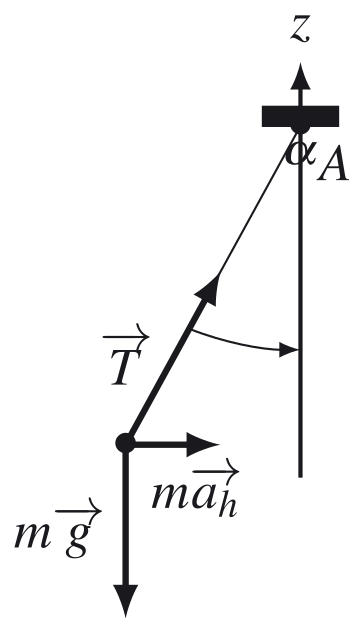
\includegraphics[width=\linewidth]{grue_corr}
			\end{center}
		\end{minipage}
	}
\end{blocQR}
\end{document}
